\documentclass{edger}
%% Preamble for EDGER paper
% PACKAGES
\usepackage{color,graphicx,subcaption,float,listings,wrapfig}
\usepackage[inline]{enumitem}
\usepackage{mathtools,commath,amssymb,cancel,siunitx}
\usepackage{xcolor,hyperref,comment}
\usepackage[normalem]{ulem}
\usepackage[noabbrev]{cleveref}
\usepackage[perpage]{footmisc}
\usepackage{lineno}
\usepackage{xcolor,soul} % for highlighting text
\usepackage{marginnote,ragged2e} % <-- used for margine notes
\renewcommand*{\raggedleftmarginnote}{\RaggedLeft}
\renewcommand*{\raggedrightmarginnote}{\RaggedRight}

% MY COMMANDS
\newcommand{\tmpcite}[2]{\texttt{[#1\footnote{#2}]}} % <-- temporary cite with a link to the source
\newcommand{\update}[1]{\textcolor{blue}{#1}} 
\newcommand{\rethink}[1]{\textcolor{orange}{#1}} % <-- command for an update that is needed
\newcommand{\instruction}[1]{\marginnote{\scriptsize{\textcolor{red}{\noindent #1}}}} %<-- instuction
\newcommand{\ilinstruction}[1]{\textcolor{red}{[#1]}}	% <-- in-line instruction
\newcommand{\spinstruction}[2]{\noindent\textcolor{red}{\hrulefill \\ \instruction{#2} #1 \noindent\hrulefill}} % <-- specific instruction
\newcommand{\moredetails}[1]{\textcolor{magenta}{#1}}
\renewcommand*{\thefootnote}{(\arabic{footnote})}     % <-- adds parantheses around footnote numbers
\newcommand{\D}[2]{\frac{D#1}{D#2}}
\newcommand{\vel}{\mathbf{v}}
\newcommand\numberthis{\addtocounter{equation}{1}\tag{\theequation}}

% MY ENVIRONMENTS
\newenvironment{tight_enumerate}{
\begin{enumerate}[label=\textbf{(\arabic*)}, ref=\arabic*]
  \setlength{\itemsep}{0.4em}
  \setlength{\parskip}{-0.25em}
}{\end{enumerate}} 
% MY COMMANDS -- editing instructions {
%\input{my-annotations}
% to learn more about the difference bewteen \input{} and \include{} see: https://www.sascha-frank.com/input_and_include.html
%}

\usepackage{myAnnotations}

\graphicspath{{figures/}}

% # Add the possibility of more sectioning {
\makeatletter
\renewcommand\paragraph{\@startsection{paragraph}{4}{\z@}%
            {-2.5ex\@plus -1ex \@minus -.25ex}%
            {1.25ex \@plus .25ex}%
            {\normalfont\normalsize\bfseries}}
\makeatother
\setcounter{secnumdepth}{4} % how many sectioning levels to assign numbers to
\setcounter{tocdepth}{4}    % how many sectioning levels to show in ToC

% Links used to implement this solution: 
% - https://tex.stackexchange.com/questions/344993/referencing-subsubsection-is-not-working-as-intended
% - https://tex.stackexchange.com/questions/60209/how-to-add-an-extra-level-of-sections-with-headings-below-subsubsection/60218#60218
% }

\begin{document}
\subsubsection*{Manuscript text color legend}
In the manuscript below, I use different styles and colors to express thought, instructions to myself, and ideas about what I think the manuscript needs to improve. This paragraphs shows examples of these styles, and should provide a \emph{'legend'} of the used styles while reading the manuscript. First, I use \tempcite{temporary citation.}{Where this footnote provides additional information about the unformulated citation mentioned in the text, or an instruction to provide a citation about a specific topic discussed without proper references.} as a note that this is a temporary citation that needs further refinement. Second, I use \ilinstruction{inline self-instructions within the text.} These inline self-instructions are meant to be intrusive and exist inline with the rest of the manuscript text to draw maximum attention. Other types of self-instructions that I use are \spinstruction{specific instruction}{Where more details are provided here}, and margin instructions that are associated with the following asterisks \instruction{This is an example of a margin instruction}. Third, I use a style that changes the color of some text, \moredetails{in order to highlight the need of more details.}
\pagebreak
\thispagestyle{plain} % defines the stye for THIS page (1st page)

\edgertitle{Fracture Detection and property estimation in microCT Images}
\shorttitle{Fracture Properties}
\edgerauthor{Omar Alamoudi (supervised by Dr. Nicola Tisato)}
\institution{}

\begin{edgerabstract}
MicroCT imaging is an exciting field when used to image experiments on rocks. A more exciting approach is imaging experiments on rock samples repeatedly over time. This allows us to 'visually' inspect the samples as the experiment progresses. Considering hydraulic conductivity as a subject of interest, particularly understanding how fracturing a rock sample under a deformation regime affects its permeability, detecting and measuring fracture properties is fundamental.

To detect and measure fracture features from microCT images of a rock sample that is evolving, a repeatable, semi-automatic workflow is required to produce consistent measurements of time variant images. Here we evaluate a Hessian filtering technique on 3D microCT images of synthetic images of fractures, and microCT images of a rock sample. We find that the Hessian filtering is successful in enhancing and detecting fractures. In addition, this technique eliminates the beam hardening effect on microCT images of rock samples which increases the reliability of picking isosurface values used in computing fracture surface area. 
\end{edgerabstract}
% ^^^ all above is not for this document

\section{Introduction}
In applications that utilize and depend on understanding multi-phase composite material properties, understanding the effects of apparent properties is generally a good approximation of how the composite behaves. It is also important to understand how the variation of the composite constituents affect said properties. The behavior of composites varies under the influence of different physical and chemical processes. For example, a primary feature that helps in understanding how composite constituents affect one another pertains to their interaction along boundaries of contact. Rocks, soils, and rock melts are three composite material examples that geologist, geophysicists, and engineers want to understand. Rocks are composed of a multiple material phases. A rock sample is composed of at least two material phases: a solid, and a fluid phase. Considering a rock sample with an economic fluid as its fluid phase, the interaction between that fluid and the rock solid phase is governed by the physical properties of each phase, the conservation of mass, momentum, and energy of their system, and the geometric distribution of these phases in the rock sample. Also, subjecting the sample to a deformation field, causes the geometric distribution to change, which perturbs the balance law quantities. With this broad view points in mind, I am interested in better understanding the processes governing fluid flow within fractured rocks under a deformation regime. The question of how fluid flow is affected by the induction and evolution of fractures in such rocks is of particular interest. 


Since fluid flow is generally dominated by flow through fracture \citep{Zoback2007} \tempcite{Zimmerman 1996, Ketcham 2005?, ...}{Add more citations stating fluid flow through porous media is dominated by fluid flow through fractures, I remember Ketcham's paper about the Inverse Point Spread Function makes the same assertion}, fracture geometric properties are primary influences on the fluid flow. An intuitive property to consider here is the fracture aperture \citep{Zimmerman1996}. Other properties such as the fracture volume, and fracture surface area are also important but are more difficult to measure \citep{Zhao2020}.  Additionally, the evolution of these fractures due to deformation is relevant to understanding the change in fluid flow in a fractured sample. For example, it is well known that the production of hydrocarbons from fractured unconventional reservoirs have a significantly higher production decline rate. This can be attributed to the closure of the artificial fractures due to mechanical or chemical healing \citep{Kleinberg2018} \tempcite{more citations needed}{add citations regarding the steep decline in production of unconventional reservoirs and its attribution to mechanical or chemical healing}. In order to understand how these properties affect the fluid flow, we need to detect and measure these fracture properties through time while under stress.

In order to understand how the evolution of fractures influences samples permeability, we plan in the near future to conduct tri-axial testing of cylindrical rock samples while simultaneously acquiring micrometer-scale Computed Tomography images (microCT), permeability measurements, and ultrasonic P and S wave velocities at multiple time instances of the experiment. A time-sequential acquisitions of these data will provide us the means to capture the effects of fracture induction and evolution on the fluid flow. The acquisition of these data types will be conducted at the same target deformation stages. Therefore, we need a systematic, semi-automatic approach to reliably and consistently detect and measure the fractures of the samples. In this paper \begin{enumerate*}[label=\arabic*)] 
\item we describe a methodology to enhance fractures in microCT images in order to measure their properties. This methodology utilizes Multi-Scale Hessian Fracture Filtering (MSHFF) technique \citep{Voorn2013}; 
\item \spinstruction{additional work needed}{Started working on this, but encountered some issues with the software Blob3D. This is not a very difficult problem to work  on, all I need to do is measure the fracture using IPSF method, which will give me a mean fracture aperture, and compare the resultant permeability using the cubic model, and compare it with the trend of permeability measurements acquired by Carolyn} Utilized the Inverse Point Spread Function method (IPSF) to measure the fracture aperture of a shale rock sample \citep{Ketcham2010}; 
\item Compare permeability measurement of said sample with the predicted permeability values based on the measured fracture aperture; 
\item describe a methodology of measuring the surface area of fractures from microCT images.\end{enumerate*}

%\begin{comment}
\subsection{Relating permeability to simplified geometries of fluid conduits}
\moredetails{The following paragraph discusses how fracture geometries have in the past been related to permeability.}
When considering a fractured, porous, and permeable rock, the fluid flow occurs predominantly through the fractures. This is an intuitive understanding of the flow given that flow through the fractures encounters the least resistance. That means that there are multiple fluid flow regimes occurring simultaneously, a Darcy fluid flow through the porous solid, and a Stokes (or Navier-Stokes) flow through the fracture \spinstruction{not sure which type of flow}{I am not sure what other types of flows are expected inside a fractured rocks. I need to establish that with some other references. I might also need some mathematical formulation, read what I learned in Ronny Borja's class Poromechanics lecture notes 1 about relating Darcy velocity to fluid flow velocity}. This distinction is not usually made clear in the literature because different research group usually refer to capacity of a fracture to conduct fluid as permeability \citep[p. 6]{Orangi2011} \tempcite{more citations needed}{The references cited here should use the term fracture-permeability even though the fractures of interest contain noting (void space)}. But Darcy permeability is only concerned with fluid flow through a porous rock sample \tempcite{original Darcy, literature on fluid flow through conventional reservoirs}{Citations properly using Darcy permeability to characterize conventional reservoirs where the predominant flow is a Darcy flow}. Therefore, it is a misnomer to discuss the permeability of the fractures but it is rather reasonable to characterize the pereability of a fractured rock as a whole. In addition, using Darcy's hypothesis to estimate fracture-permeability under estimates the permeability of the fractured rock \citep{Singh2019}. This is of course because fluid flow through a fractured rock occurs mostly through the fractures rather than the porous matrix surrounding it. A simplified model of a non-porous solid with a void with known geometry through which the fluid flows helps us understand how void geometrical properties affect the fluid flow. Two geometries are discussed below: a cylindrical void inside a cylindrical sample, and a plate-like void splitting a cylindrical sample.

\subsubsection{Cylindrical void model}
Darcy's law shown in \autoref{eqn:Darcy's Law} \citep{Darcy1856} governs the conductivity of fluid within a cylindrical porous material sample with known geometry. The driving force of the fluid motion is the pressure gradient. Darcy's law does not make any explicit declarations about the spatial distribution, or shape of the pores within a rock specimen. On the other hand, the Kozeny--Carman \citep{Carman1961, Mavko2009} describes the fluid flow through a cylindrical cavity in solid block see \autoref{eqn:Kozeny-Carman}. Imagine drilling a cylindrical cavity in the cylindrical sample with the known geometry with Radius R. \Autoref{eqn:Kozeny-Carman} describes the flow through that cavity. 

\begin{equation}
Q = - \frac{A}{L} \frac{\kappa }{\mu} \Delta p \label{eqn:Darcy's Law}
\end{equation}

\begin{equation}
Q = - \frac{1}{L} \frac{\pi R^4}{8\mu} \Delta p \label{eqn:Kozeny-Carman}
\end{equation}

\begin{equation}
\kappa = \frac{\pi R^4}{8A} \label{eqn:perm}
\end{equation}
Comparing \autoref{eqn:Darcy's Law} and \autoref{eqn:Kozeny-Carman}, \autoref{eqn:perm} shows that there is a correlation between the sample fluid permeability, the cross sectional area of the sample, and the radius of the cavity. Considering an alternative case where we have fractures, one can deduce that we can estimate or predict the relationship between a rock sample geometry and fractures within the sample that would be the primary conduit of fluid flow. Therefore, the use of microCT images to map fractures is an important first step to understanding such relationship. 

Considering a single two-dimensional slice from a three-dimensional microCT volume data of two half-cylinder of a rock sample, \cite{Ketcham2010} have demonstrated the applicability of what the authors call the Inverse Point Spread Function method (IPSF) in measuring the apparent and true aperture of fractures from microCT volumes. Using this method requires visually inspecting and detecting the fractures in the image, then measuring them. An alternative approach proposed by \cite{Voorn2013} employs computing the Hessian to detect multi-scale fractures within a sample. In the paper, we discuss the application of \cite{Voorn2013} approach on synthetic images as a first step in attempting to detect fractures with the aim to eventually measure them. We also attempt to estimate fracture surface area of a cylindrical sample that was subject to a rotary shear experiment \citep{Zhao2017}. MicroCT images of the samples were acquired before and after fracturing.
%\end{comment}

\subsubsection{Plate-like void splitting a cylindrical sample}
\moredetails{I need to add the model that is based on Zimmerman's 1996 work here. The work that was in my proposal.}

\section{Materials and Methods}
	Our main objective is to improve the ability to detect, and henceforth measure fractures in microCT images acquired of rock samples. The developed method must be systematic, semi-automatic, and generates reproducible results \tempcite{cite reproducebility papers}{I value reproducibility, and there is a significant amount of research stating is value. Fomel's group does this as well as Stanford Exploration Project SEP}. The necessity of the systematic analysis in detecting and measuring fractures is due to our over arching goal to use the developed methodology to measure the evolving fracture properties in microCT images over time of a sample undergoing deformation and fracturing.  

\subsection{Fracture Detection and Measurement}
	As a first step, we enhance the images of fractured rocks, after which we attempt different approaches of measuring the fracture properties in the enhanced images. The methodology used is based on \cite{Voorn2013}. \spinstruction{An idea}{I need to consider using the Laplacian $\Delta = \nabla \cdot \nabla G(\mathbf{x})$ as a filter. Because the Laplacian provides a measure of how different a surround area is to the point at which the Laplacian is evaluated.} \tempcite{convolution as a proxy for derivatives}{Cite papers that show that convolving the hessian of the Gaussian with an image with different scale factor $s$ is equivalent to taking the spacial derivative. I think a first place to start looking for this is the citations in \cite{Voorn2013}, and medical papers pertaining to geometric features of bones etc. in microCT images} To demonstrate this approach in detecting fractures, we first apply the methodology on two-dimensional (2D) and three-dimensional (3D) synthetic images. I generated these images with basic geometric features resembling fractures. I then computed the spatial Hessian matrix for each voxel of the synthetic images, and finally conduct further analysis to map the fracture like features. The description of these steps follows in the same order stated. 

\subsubsection{Synthetic Image Generation} \label{sec:Synthetic Fractures}

\begin{figure}[!h]
\centering
    \begin{subfigure}[b]{0.5\textwidth}            
            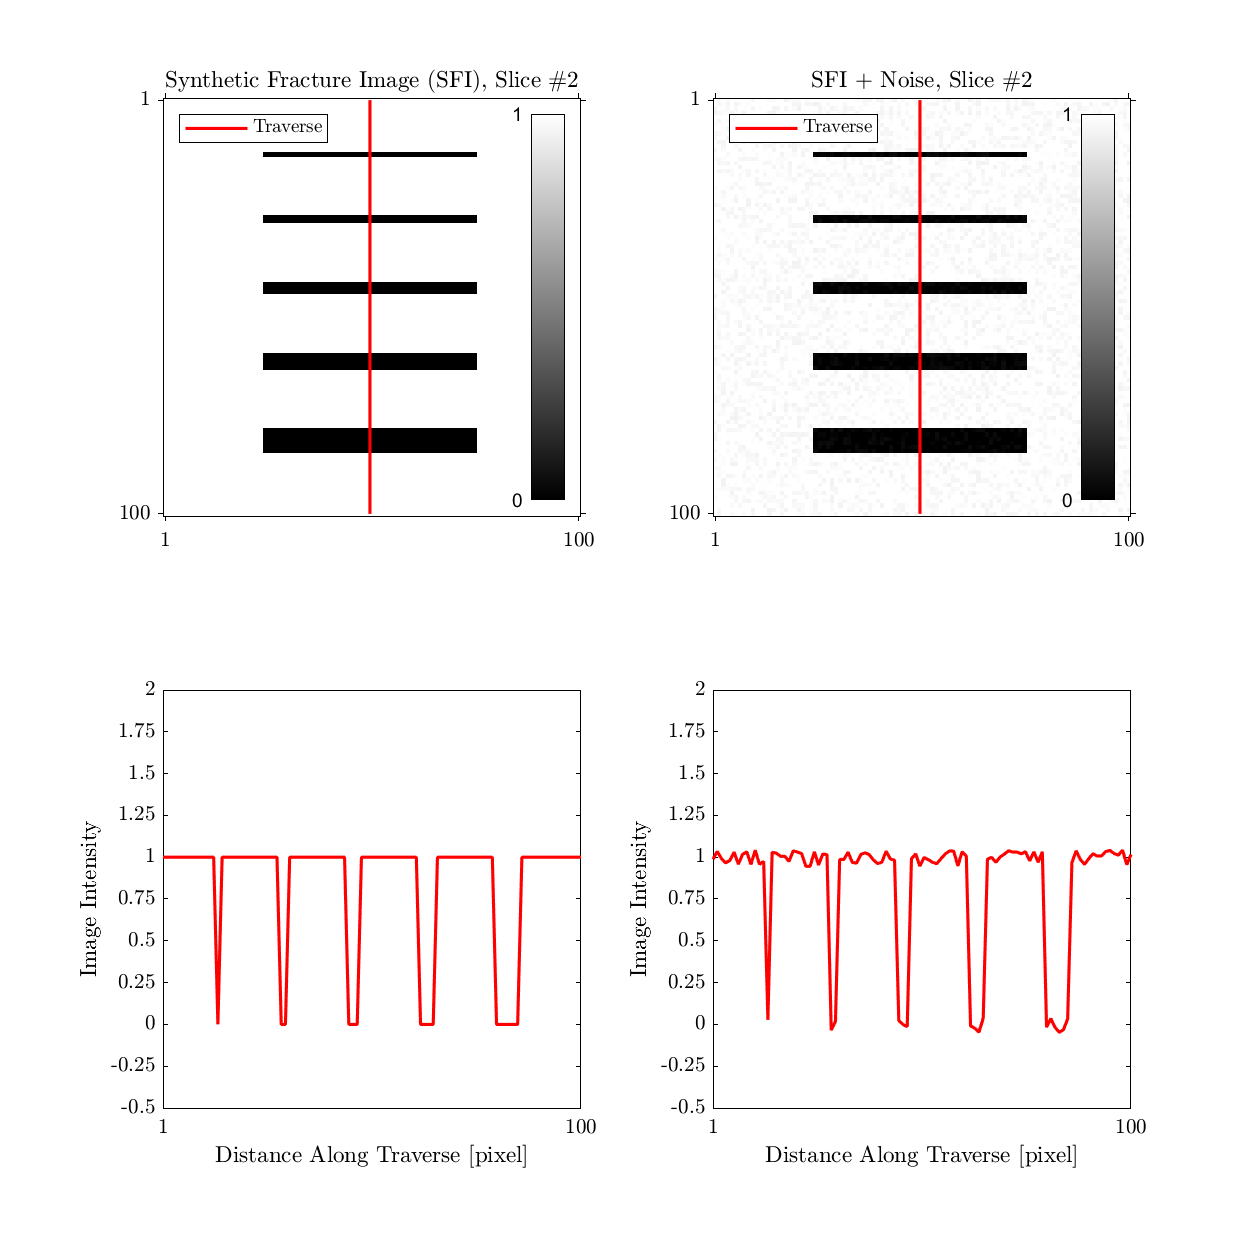
\includegraphics[width=\textwidth]{3DSyntheticFractureImages.png}
            \caption{Set of "sharp" images}
            \label{fig:Sharp images}
    \end{subfigure}%
     %add desired spacing between images, e. g. ~, \quad, \qquad etc.
      %(or a blank line to force the subfigure onto a new line)
    \begin{subfigure}[b]{0.5\textwidth}
            \centering
            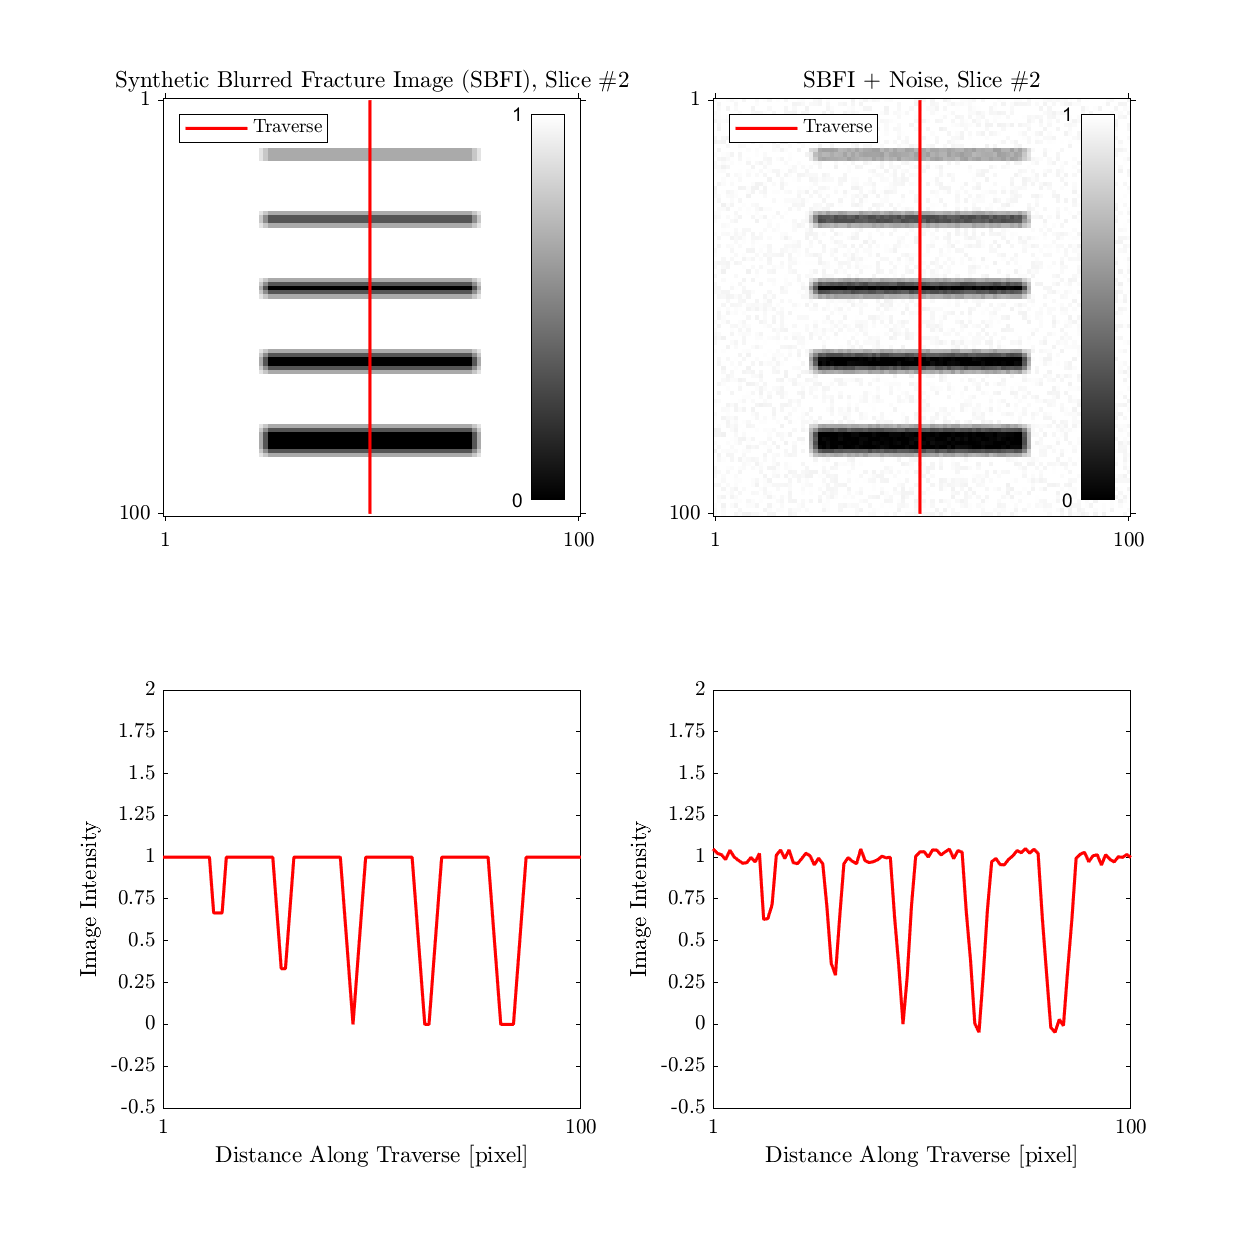
\includegraphics[width=\textwidth]{3DSyntheticBlurredFractureImages.png}
            \caption{Set of blurry images}
            \label{fig:Blurry images}
    \end{subfigure}
    \caption{The middle slice of a three-dimensional synthetic images. Top row shows the images, and the bottom row shows a traverse along the vertical red line. }
    \label{fig:Synthetic images}
\end{figure}

The workflow used in generating the synthetic fracture images was done using Matlab. The objective of creating these images is to calibrate the outcome of analysis that will be discussed later in \autoref{sec:EnhancingFractturesInMicroCTImages} and \autoref{sec:MeasuringFractureSurfaceArea}. A function was created that takes four input parameters and generates a synthetic image of a white background and black rectangles, for 2D images, and cuboids for 3D images. The input parameters are: (1) the length a long the x and y axis of the square synthetic image; (2) an array of integers representing the fracture apertures in pixels/voxels, i.e. \texttt{[1,2,3,4,6]}; (3) a boolean flag specifying if random noise should be added to the image; (4) and a signal to noise (SNR). For every function call, an equally spaced vertical fractures are drawn into an image as pixels with the value zero in a background of value one. The resultant image is a square image with an edge length specified by the first input argument see \autoref{fig:Synthetic images}. 

In order to understand the effects of blurring and noise in our analysis, four different images are generated using identical image size and fracture apertures in two sets. The first set is of two "sharp" images, and the other two are blurred images. The blurring is produced by the convolution of the sharp image with a 3-by-3 (-by-3 in 3D) box filter. The blurred images are a rudimentary attempt to represent the effect of the Point Spread Function (PSF) of a microCT machine \citep{Ketcham2010}. In each set, one image is noise free while random noise was added to the other. This is our attempt to observe and quantify the effect of random noise. The result of this workflow is images with the specified fracture apertures as the apparent fractures. Since our objective is to map fractures, a plate like geometrical features, \cite{Voorn2013} have stated that two-dimensional images are insufficient in mapping fractures.  To generate 3D images with fractures that are vertically oriented, a stack of three identical images are superimposed on one another. For the images that contain noise, three different realizations of noise are stacked to preserve the randomness of noise. \Autoref{fig:Synthetic images} shows the middle slice of a three-dimensional image with input parameters [1,2,3,4,6] for fracture apertures, 100 voxels for the length of the image, and 10 for the SNR. 

\subsubsection{MicroCT Images and Sample Description}

\begin{figure}[!h]
\centering
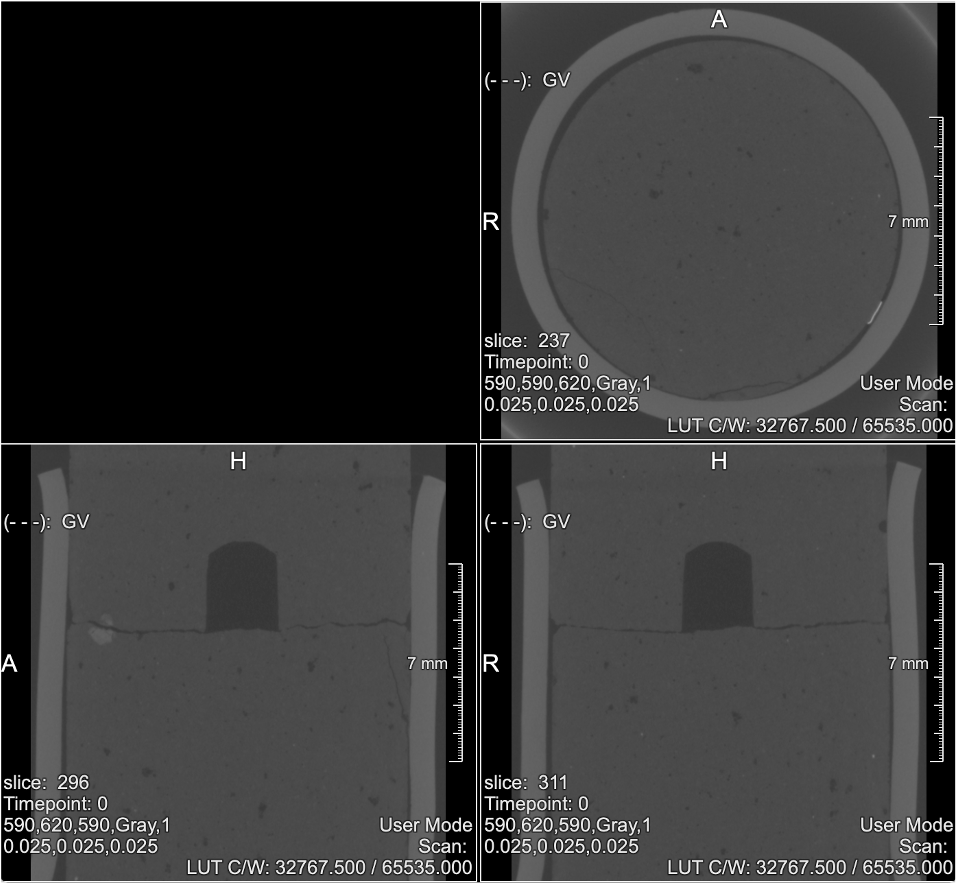
\includegraphics[width=0.4\textwidth]{0_degreeOrthoView.png}
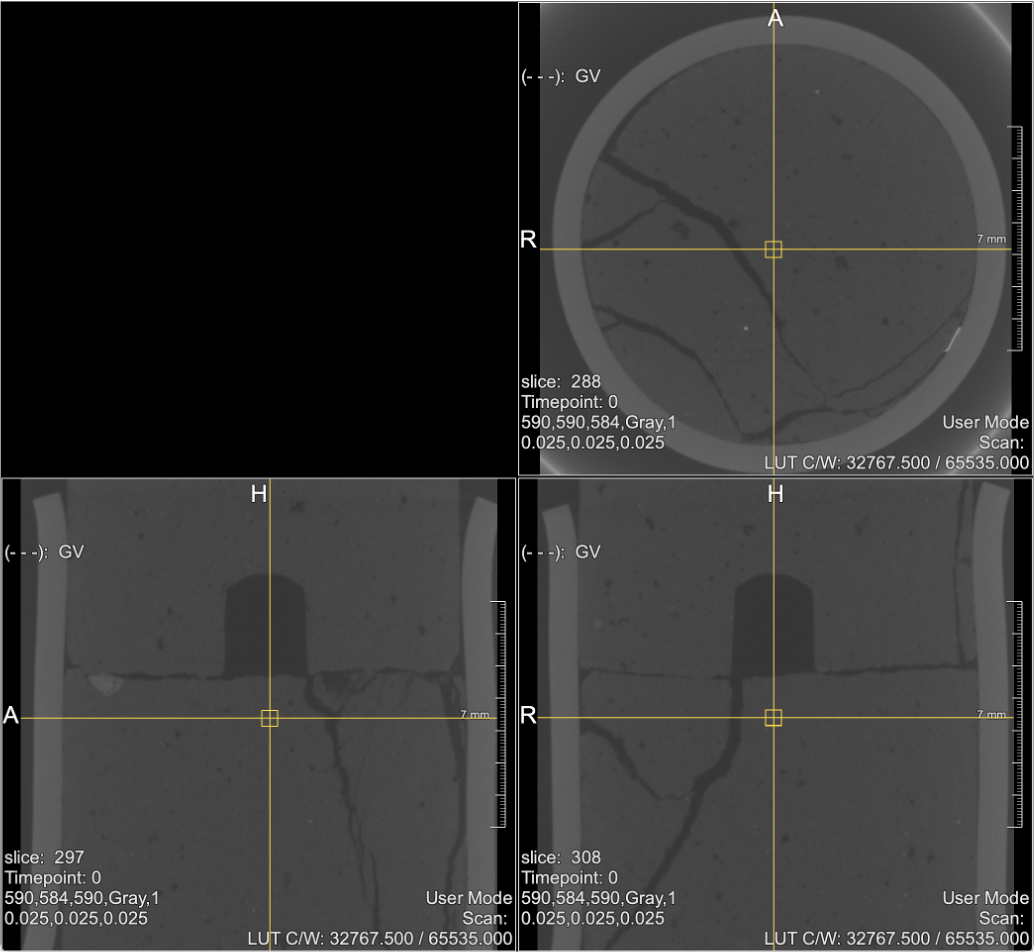
\includegraphics[width=0.4\textwidth]{18_degreeOrthoView.png}
\caption{An orthogonal view of the images 0\_degree (left) and 18\_degree (right). This view is generated using the 'OrthoView2D' of MeVisLab software. Both semi-samples are shown. The top semi-sample shows the cavity. Fractures shown are a result of rotating the top semi-sample while applying normal force. }
\label{fig:18Degree}
\end{figure}

In \autoref{sec:Enhancing Fractures in microCT Images Using Hessian Filtering}, we apply a Hessian filtering technique to enhance fractures in microCT images or rocks. We utilized The microCT images used were available through \cite{Zhao2020} and described in \cite{Zhao2017,Zhao2020}. In summary, the image volume comprises 1024 slices a long the z axis, and 794 voxels along the x and y axes. Each voxel holds a 16-bit gray value corresponding to approximately the amount of X-ray attenuation incurred by the material in that voxel. The voxels are isotropic cubes with edge length of 25micrometer. 

The images are for a cylindrical sample that underwent a rotary shear experiment. Six 3D microCT image volumes are available. Here we use two images that were acquired at two different time steps of the experiment. The image from first time step named 0\_degree, and the image from the third time step which is called 18\_degree, see \autoref{fig:18Degree}. This provides us the means to observe difference in fracture induction in the sample over time. The scanned sample is a cylindrical flowstone sample that is 12mm in diameter and 32mm in length. After casting and curing, the sample was carefully split horizontally into two cylindrical semi-samples with a rough surface in the middle representing a horizontal fault surface. A semi-conical cavity of 2.5mm diameter and 3mm in depth was drilled into the top semi-sample. This cavity was created to eliminate the potential of the sample fracturing due to compression since the displacement of the central portion of the material is minimal. The sample was intended to fracture only due to rotary shear motion. Since the sample was attached to a stainless steel sample holder, analysis were conducted on part of the sample focused around the horizontal fault. The portion of the images closes to the sample holder was cropped out since they were heavily influence by artifacts from caused by the sample holders. The final images comprise a total of 620 slices around the horizontal fault, see \autoref{fig:Zhao2017_fig-6-7}. The number of slices used are 137-756. 

\begin{figure}[!h]
\centering
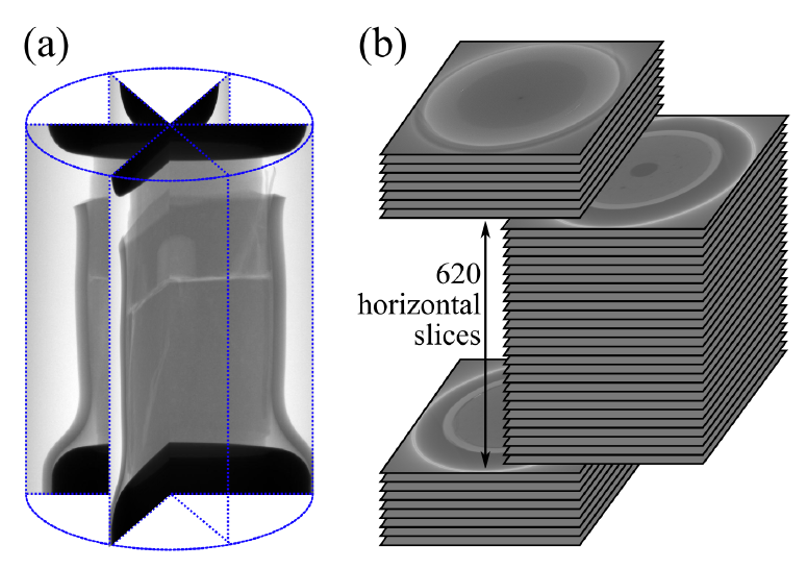
\includegraphics[width=0.5\textwidth]{Zhao2017_6-7.png}
\caption{(a) Radial cross sections showing the entire sample. (b) The cropped volume used in the analysis. After \cite{Zhao2017}}
\label{fig:Zhao2017_fig-6-7}
\end{figure}

\subsubsection{Enhancing Fractures in microCT Images Using Hessian Filtering} \label{sec:Enhancing Fractures in microCT Images Using Hessian Filtering} \label{sec:EnhancingFractturesInMicroCTImages}
\paragraph{Computing the Hessian} \label{sec:The Hessian}
To compute the Hessian of a microCT image, consider a three dimensional Euclidean domain $E^3$ representing the domain of a microCT image, and given a scalar valued field $I: E^3 \rightarrow \mathbb{R}$ representing the gray value of every voxel. The Hessian of the scalar field $I$ is $\mathbf{H}(I)$. Consider the matrix notation of the Hessian as shown in \autoref{eqn:hessian}. 

\begin{align*}
\mathbf{H} & = 
\begin{bmatrix}
I,_{xx} & I,_{xy} & I,_{xz} \\
I,_{yx} & I,_{yy} & I,_{yz} \\
I,_{zx} & I,_{zy} & I,_{zz}
\end{bmatrix} \numberthis \label{eqn:hessian}
\intertext{Where} 
I & = \text{microCT image gray value field, or image intensity} \\
I,_{ij} & = \frac{\partial}{\partial i } \left(\frac{\partial I }{\partial j} \right). \qquad i,j \in \{x,y,z\} \numberthis \label{eqn:Second Derivative of I}
\end{align*}

The Hessian is a tensor value function $\mathbf{H}: E^3 \rightarrow \mathbb{R}^3 \times \mathbb{R}^3$. It has nine components six of which are unique because the Hessian is symmetric. $H_{ij}$ denotes the component of the ith row and jth column. The indices $i,j \in \{x,y,z\}$. $x, y$, and $z$ are right-handed orthogonal coordinates of a defined Euclidean space $E^3$. Since microCT images, or digital images in general, are discrete in nature, the computation of the derivatives can be done by finite differences for example. But that is not adequate since fracture features are of different scales. Therefore, a \emph{multi-scale} technique is more useful. 

An over view of such technique is provided by \cite{Lindeberg1998}. This technique considers different scales of edge features, in our case represented by fractures. For example, the second derivative $I,_{xy} = \frac{\partial }{\partial x} (\frac{\partial I}{\partial y})$ of a three-dimensional image represented by a scalar valued function (gray value) $I = I(x,y,z)$ for every voxel with coordinates $(x,y,z)$ is computed as the convolution of the image $I$ with the second derivative of the three-dimentional Gaussian $G,_{xy}$ as following:
\begin{align*}
I,_{xy} & = \alpha \left[I * G,_{xy}(x,y,z,s) \right] \numberthis \label{eqn:I xy}
\intertext{Where}
\alpha & = \text{Normalization factor} \\
G(x,y,z,s) & = \exp\left\{ -\frac{1}{2s^2} \left[ \left(x - x_0\right)^2 + \left(y - y_0 \right)^2 + \left(z-z_0 \right)^2 \right] \right\} \quad (\text{Gaussian})\\
\end{align*}

\begin{figure}[!h]
\centering
    \begin{subfigure}[b]{0.5\textwidth}            

            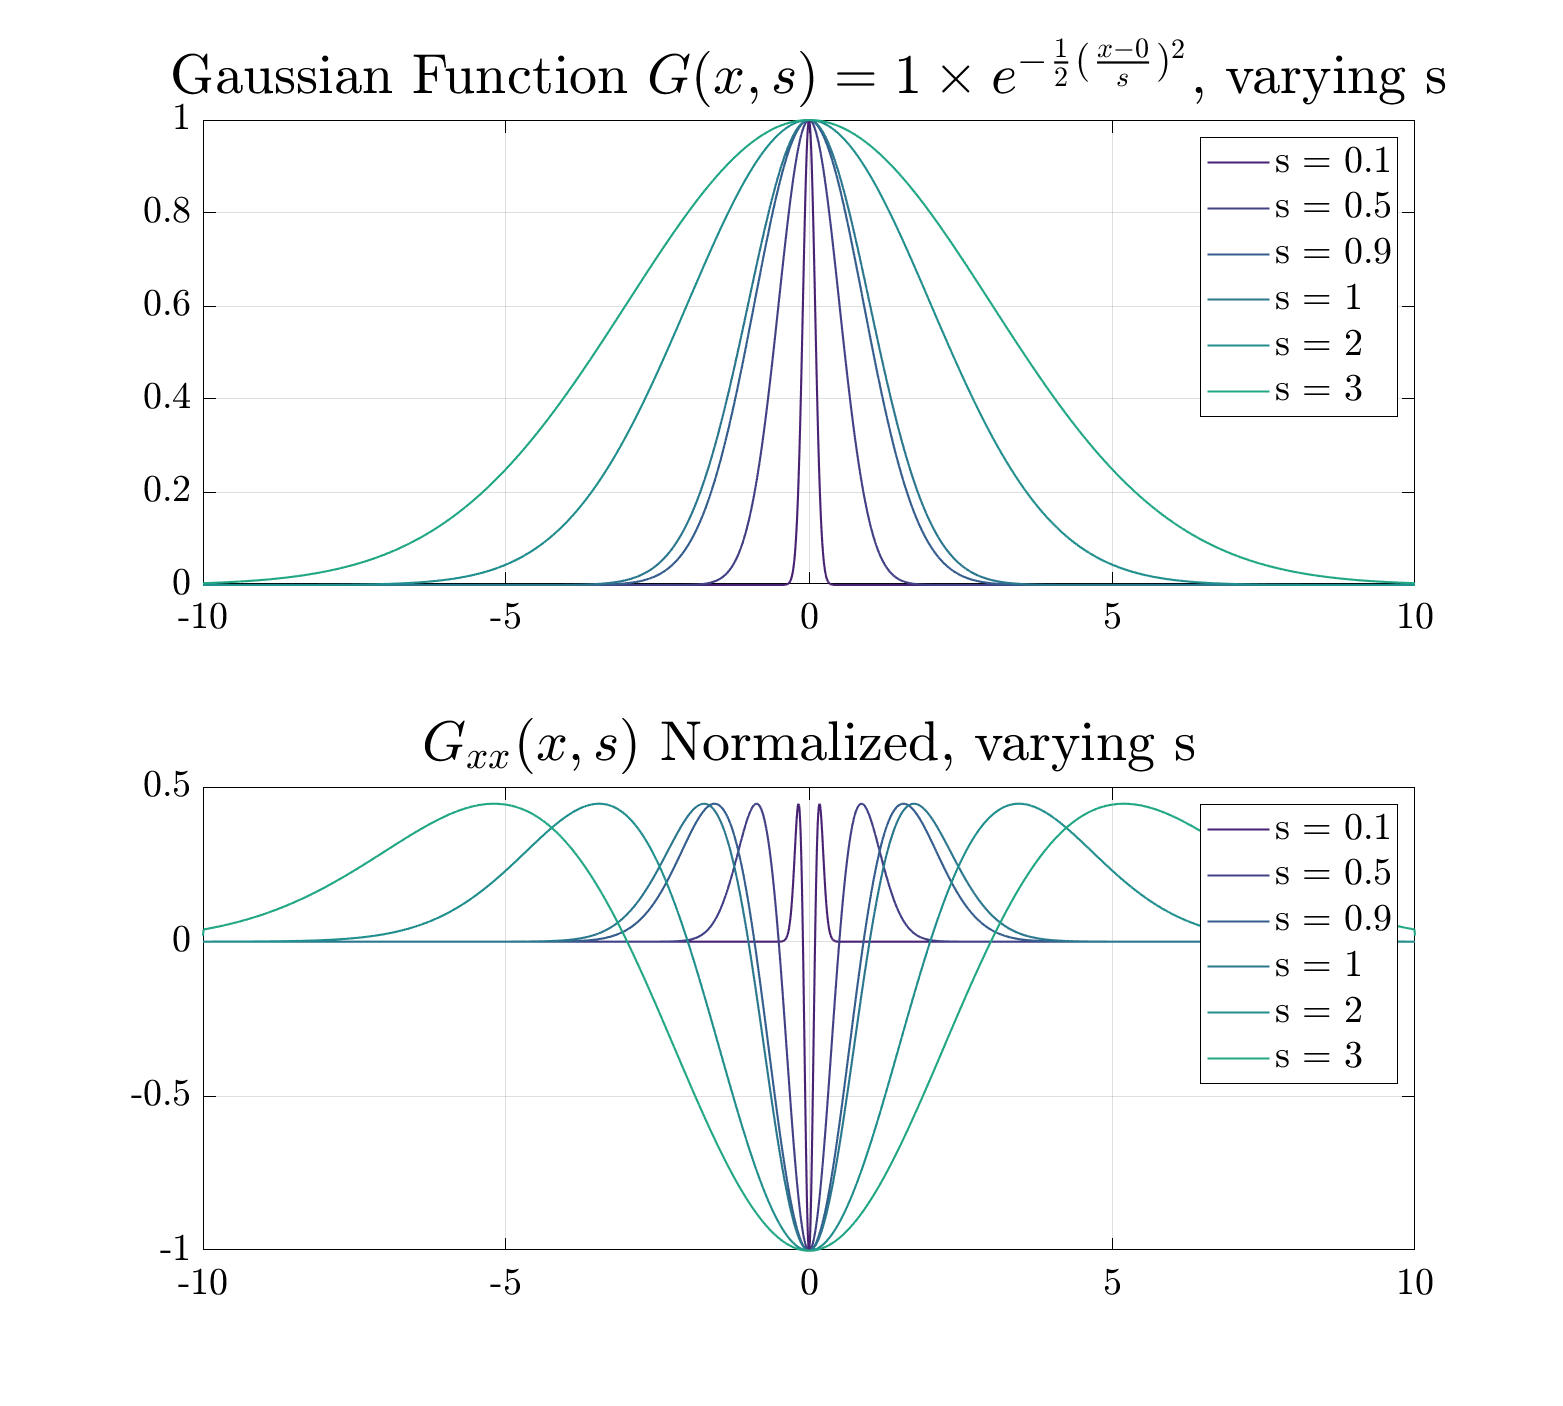
\includegraphics[width=\textwidth]{gaussian_continuous.png}
            \caption{Continuous}
            \label{fig:Gaussian cont}
    \end{subfigure}%
     %add desired spacing between images, e. g. ~, \quad, \qquad etc.
      %(or a blank line to force the subfigure onto a new line)
    \begin{subfigure}[b]{0.5\textwidth}
            \centering
            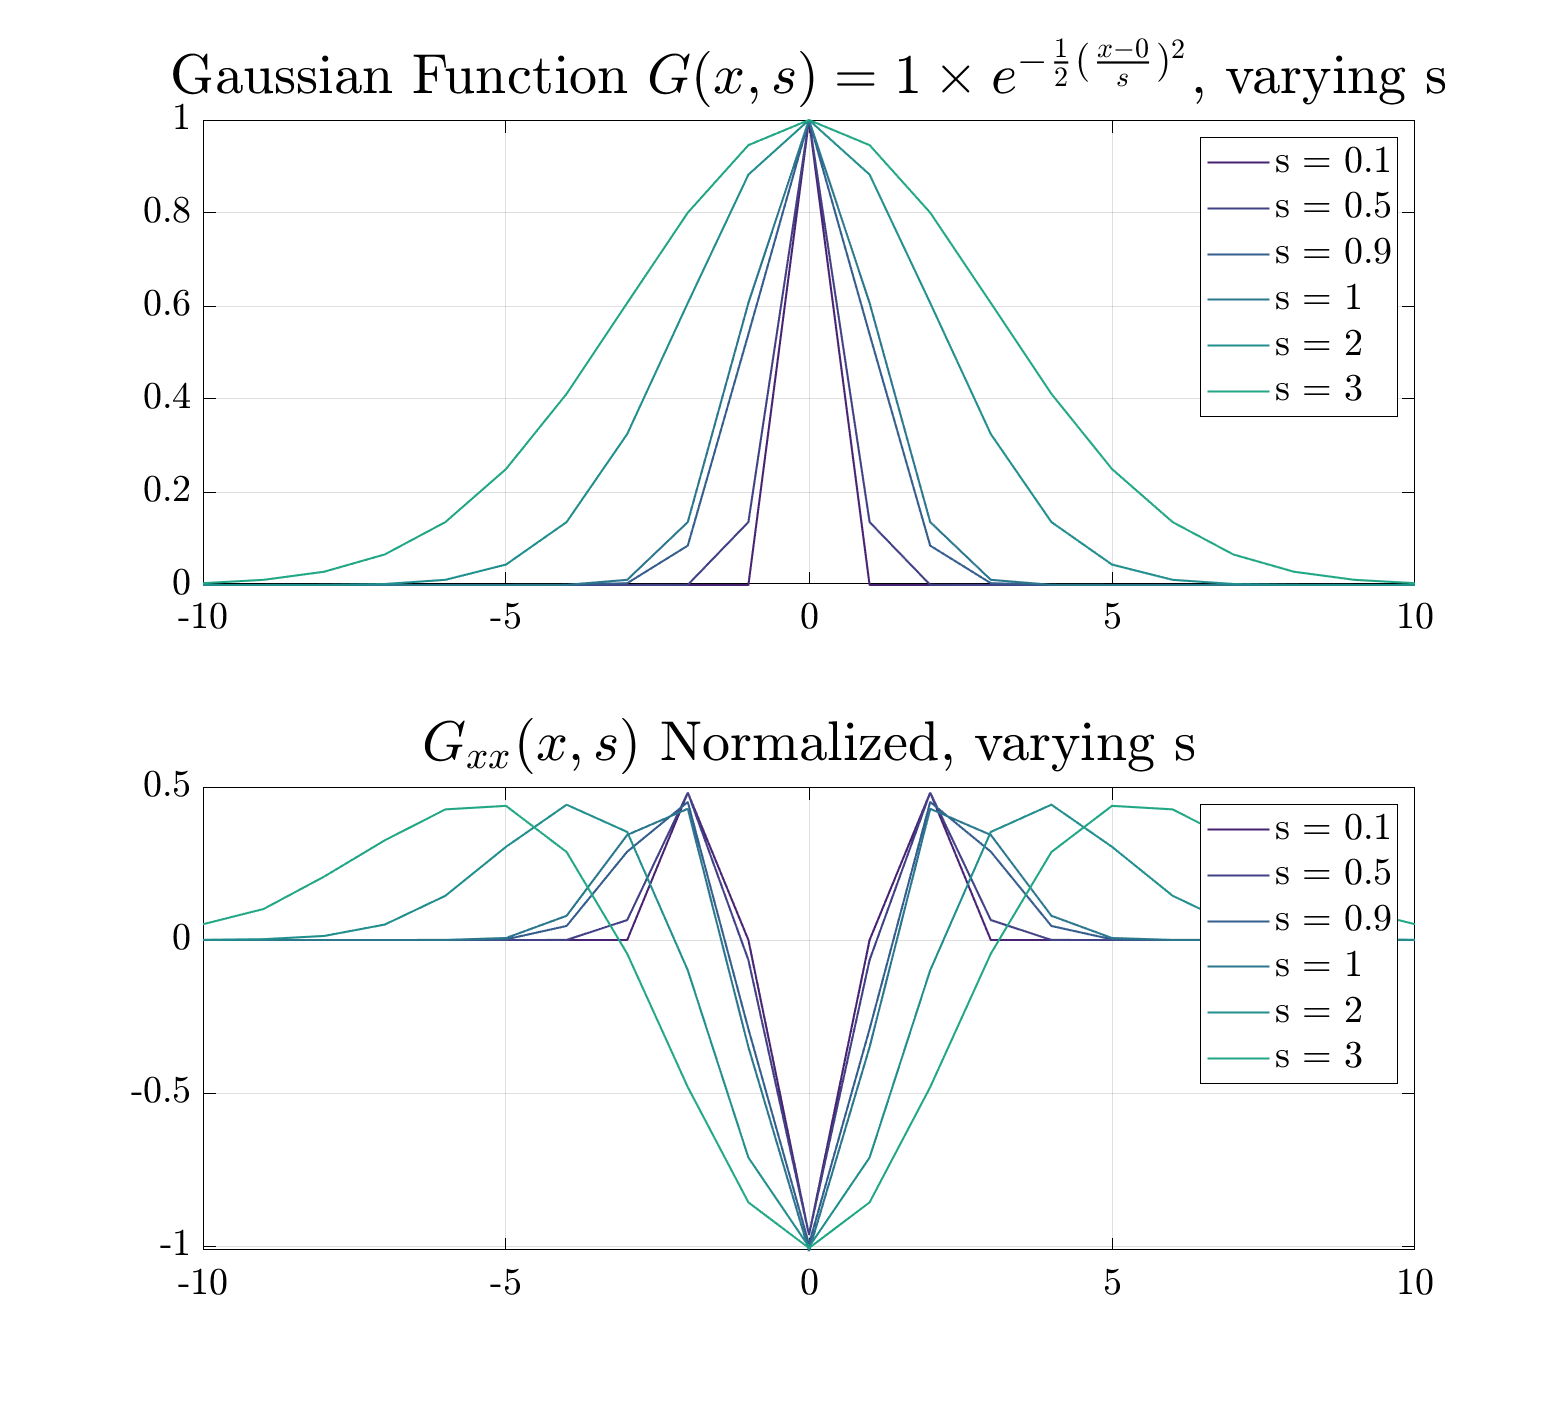
\includegraphics[width=\textwidth]{gaussian_discrete.png}
            \caption{Discrete}
            \label{fig:Gaussian disc}
    \end{subfigure}
    \caption{One-dimensional Gaussian function and  its second derivative with varying $s$ in continuous and discrete forms.}
    \label{fig:Gaussian function}
\end{figure}

\Autoref{fig:Gaussian function} shows a one-dimensional Gaussian function and the second derivative in a continuous and a discrete form. The second derivative is equivalent to the $G,_{xx}$ component of the multi-dimentional Gaussian function. This is the kernal that is convolved with the intensity of the image as shown in \autoref{eqn:I xy}. It is important to note that all of the operations carried out here is done using the discrete form. Different curves shown in \autoref{fig:Gaussian function} correspond to a different scaling parameter $s$. Darker colors correspond to small $s$, while brighter colors correspond to a larger $s$. 

For a given image, I computed all nine components of the Hessian for each voxel for different values of the scaling parameter $s$. This was done by (1) choosing a value for $s$; (2) generating the proper three-dimensional Gaussian filter $G(x,y,z)$ using the   Image Processing Toolbox function \texttt{fspecial3} with a filter size of either 18 or 19. The size of the filter was dependent on $2s$. The filter was 18 if $2s$ was even and 19 if $2s$ was odd.(3) computing the nine derivatives, $G_{ji}(x,y,x)$ for $i,j = [x,y,z]$, that are used in \autoref{eqn:I xy}, then convolving the result with the images while choosing $\alpha = 1$. Looking at the bottom plot of \autoref{fig:Gaussian cont}, each curve can be defined by it largest trough bounded by two smaller peaks. The distance that defines the largest trough for every curve between the two points (closest to zero) intersection the horizontal axis is $2s$. 

\paragraph{Fracture Enhancement Analysis} \label{sec:Fracture Enhancement Analysis}
After computing the all nine components of the Hessian for every voxel of the synthetic images for every value of $s$, we compute the eigenvalues $\lambda_1,~ \lambda_2,~\lambda_3$, where $\lambda_1 < \lambda_2 < \lambda_3$. I used the Matlab function \texttt{eig} to do so. For every value of $s$, within and close to plate like features, we expect one of the eigenvalues to have a large magnitude while the other two to have small magnitudes. Using the same criteria proposed by \cite{Voorn2013}, we can then define a new value $A_s$ for every voxel such that 
$$A_s = \begin{cases}
\lambda_3 - |\lambda_2| - |\lambda_1| &\quad \text{if} ~ (\lambda_3 - |\lambda_2| - |\lambda_1|) > 0\\
0 \qquad &\text{otherwise}
\end{cases} $$
where the subscript $s$ here denotes for the scaling parameter. We then normalize $A_s$ such that $B_s = \frac{A_s}{\max(A_s)}$, and finally define another quantity $C_s$ such that 

\begin{align*}
C_s = \begin{cases}
1 & \text{if} ~ B_s > 1 - \gamma \numberthis \label{eqn:gamma} \\
0 & \text{otherwise}
\end{cases}
\end{align*}

$\gamma$ is an arbitrary tolerance that I chose to be $0.70$ in my application. I then summed up all of $C_s$ for all scaling parameters used. In my case, since this analysis was applied to a synthetic image set, the scaling parameter was set to be $s = \frac{1}{2}  [1,2,3,4,6]$. \Autoref{fig:Fracture Mapping Analysis} shows the results of conducting the above steps for every value $s$. 

The final step is combining all different images for every value of $s$, and inverting the image to match the original synthetic image as shown in \autoref{fig:copmaring voorn}. 

\begin{figure}[H]
\centering
\includegraphics[width = \textwidth]{"SFI,s = 0.5, Aperture = 1, Frac (1 of 5), hsize = 19"}
\includegraphics[width = \textwidth]{"SFI,s = 1, Aperture = 2, Frac (2 of 5), hsize = 18"}
\includegraphics[width = \textwidth]{"SFI,s = 1.5, Aperture = 3, Frac (3 of 5), hsize = 19"}
\includegraphics[width = \textwidth]{"SFI,s = 2, Aperture = 4, Frac (4 of 5), hsize = 18"}
\includegraphics[width = \textwidth]{"SFI,s = 3, Aperture = 6, Frac (5 of 5), hsize = 18"}
\caption{From top to bottom, incremental results for every scaling value $s$. Left to right of each row $A_s$, $B_s$, $C_s$, and the cumulative addition of the current step and all of the previous ones of $C_s$. Note here that the bottom row shows the final result of the analysis before normalizing and inverting the image. }
\label{fig:Fracture Mapping Analysis}
\end{figure}


\subsubsection{Using \texorpdfstring{\cite{Voorn2013}}{Voorn et al. (2013)} Code} 
The code for the method described in \cite{Voorn2013} to enhance multi-scale fractures is available in a GitHub repository. At first, I recreated the entire workflow in Matlab with the intention of attempting to further address sub-voxel fractures with minor success not discussed here. More work is needed to achieve this objective. In \autoref{sec:results comparing my outcome and voorns} I will discuss the difference in the outcome of my code compared to the outcome of the code published by \cite{Voorn2013}. The synthetic image used in this comparison is the Synthetic Blurry Fracture Image with added noise (SBFIN) that is shown in \autoref{fig:Blurry images}. The results of using my code compared to the published code is shown in \autoref{fig:copmaring voorn}. 

\begin{figure}[!ht]
\centering
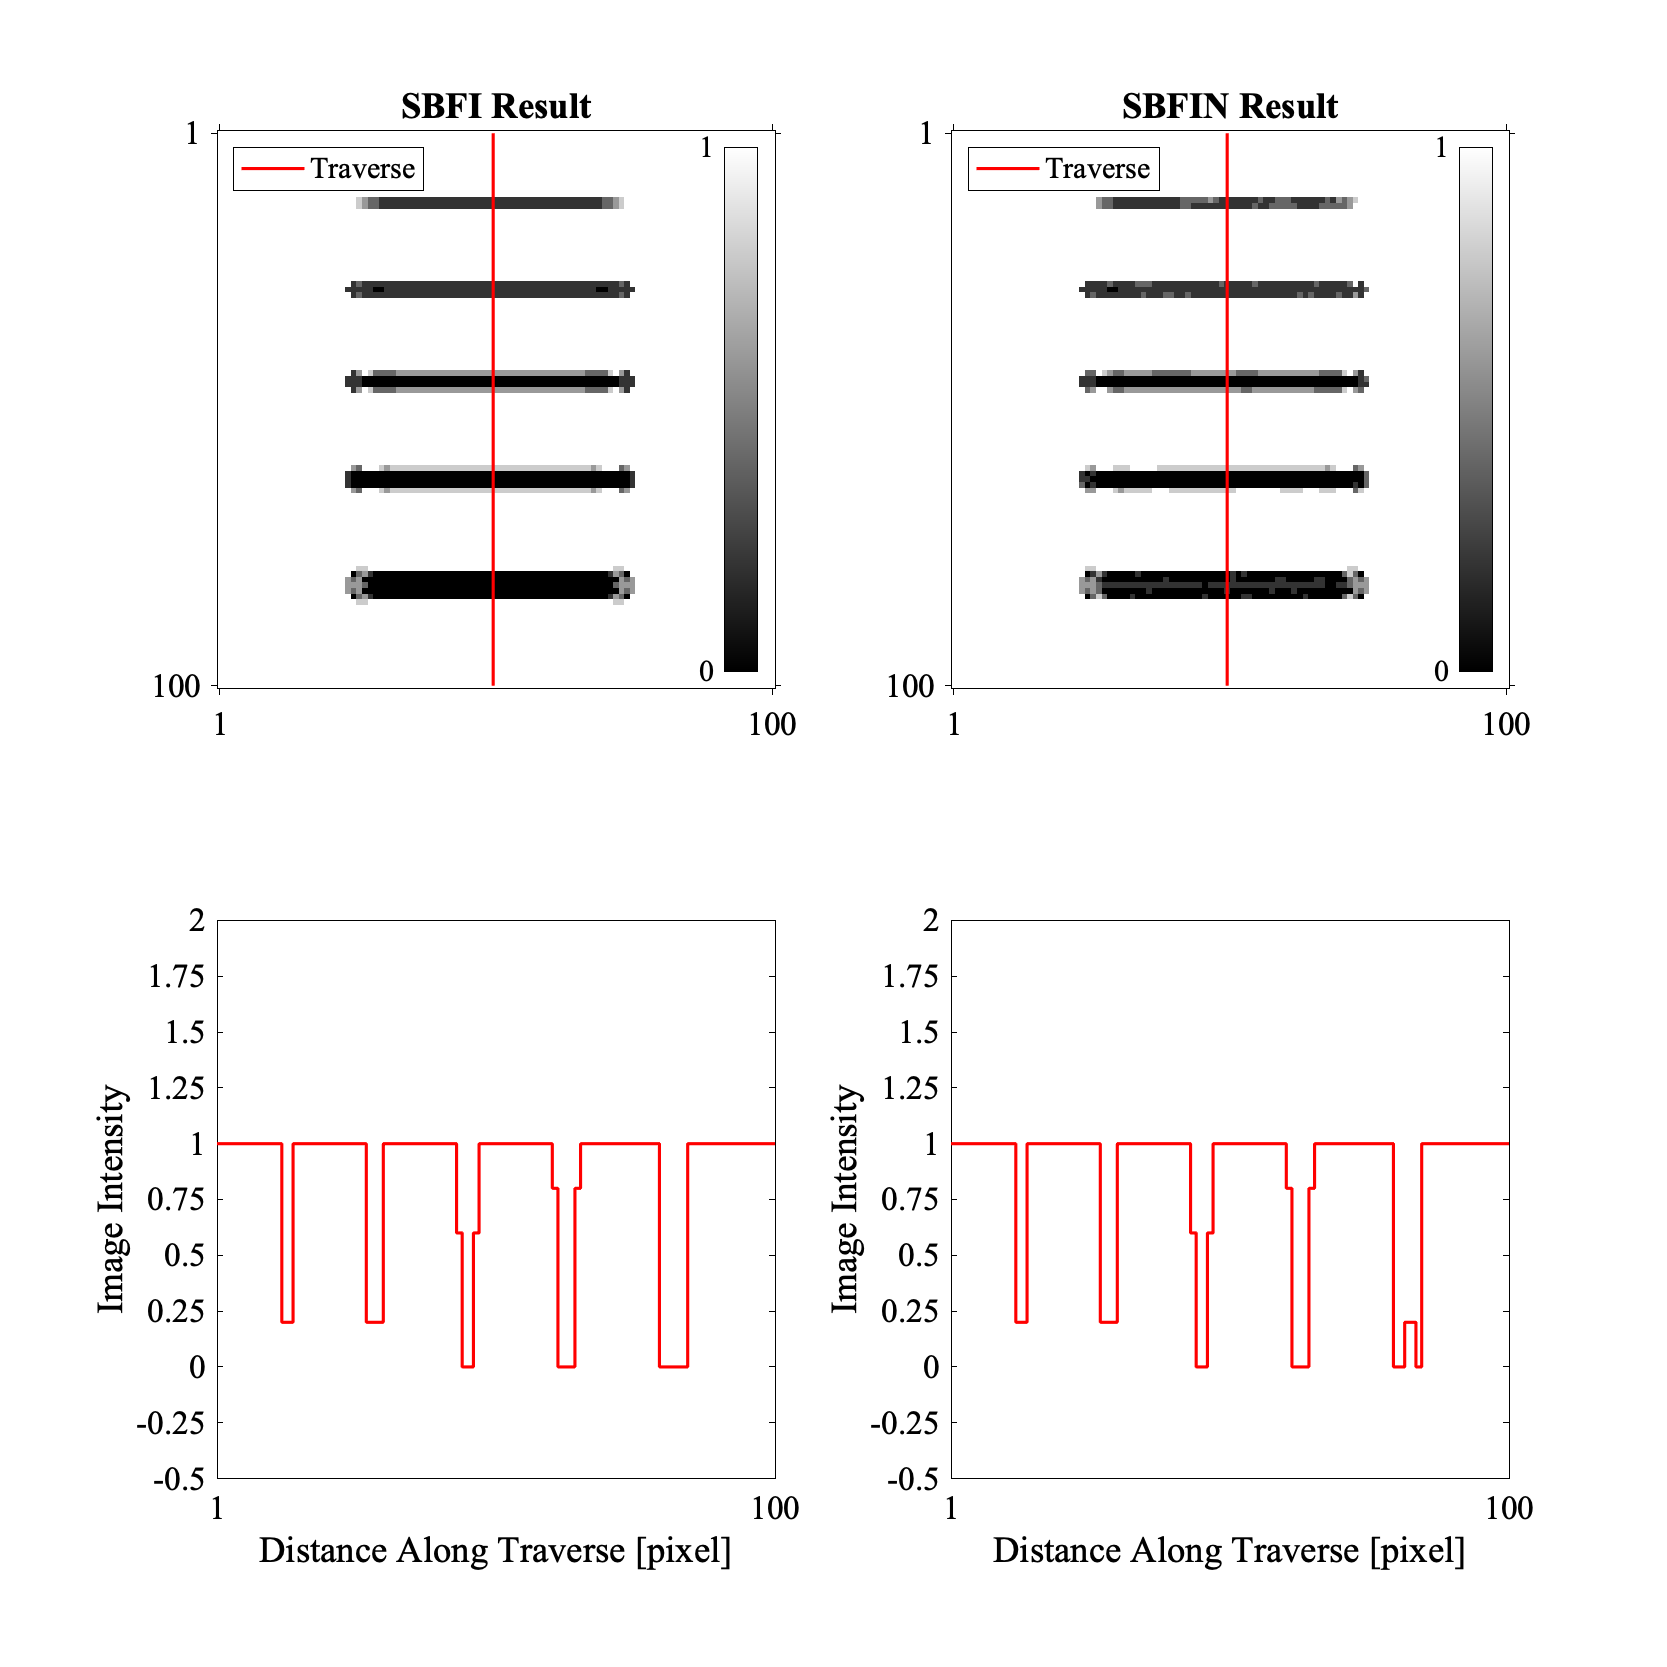
\includegraphics[width=.6\textwidth]{HessianResultsSBFI_N.png}
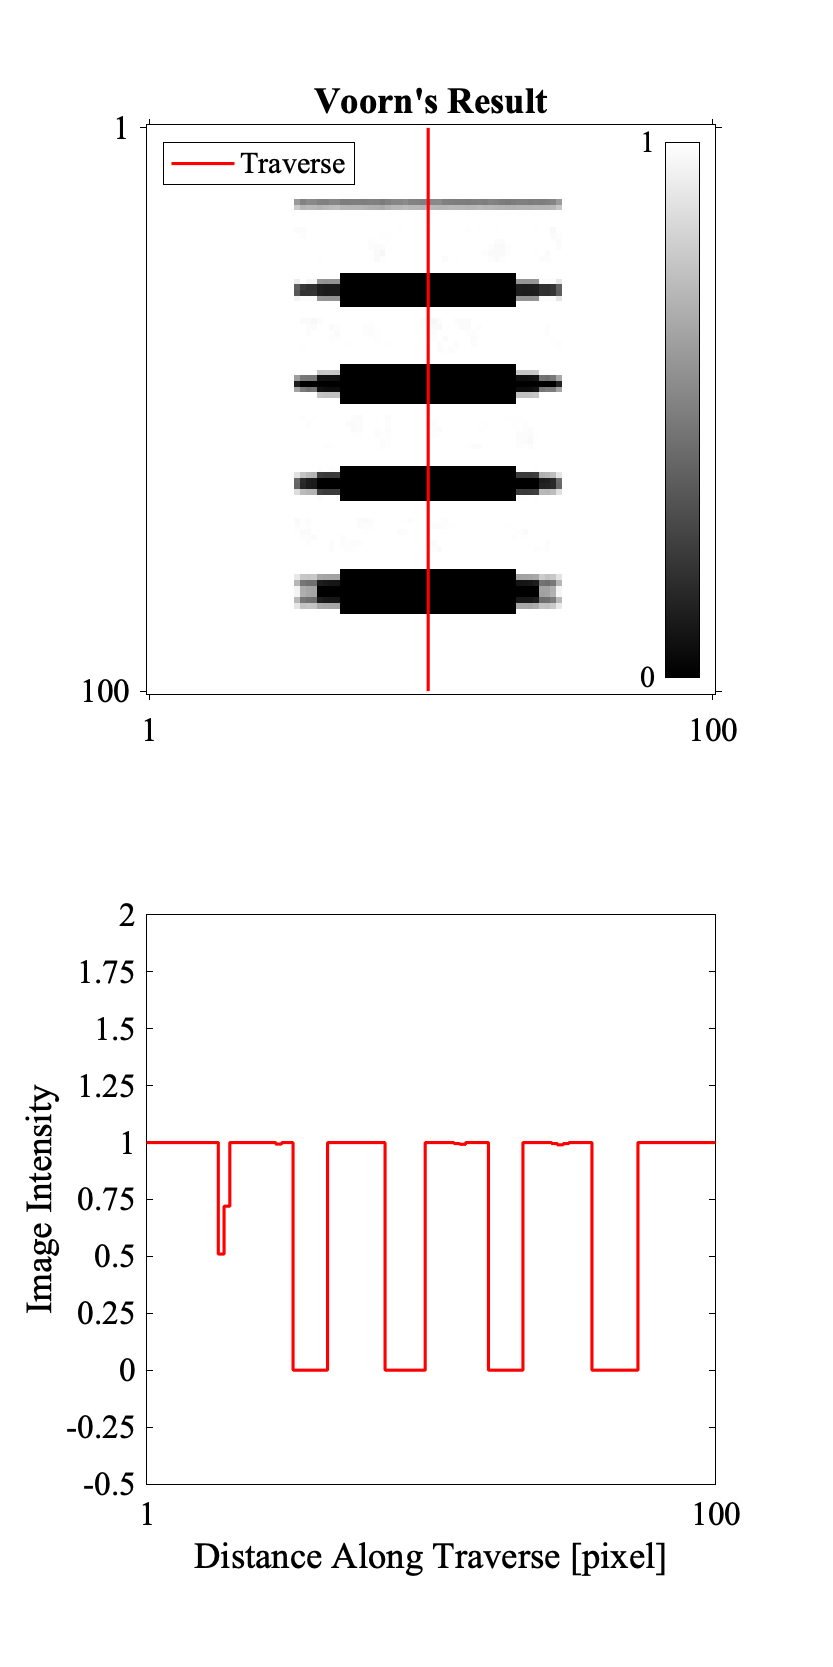
\includegraphics[width=.3\textwidth]{VoornsResults.png}
\caption{The results of using the Hessian filtering technique on synthetic fracture images. From left to right: result from my implementation on the Synthetic Blurry Fracture Image (SBFI); Result from my implementation on the Synthetic Blurry Fracture Image with Noise; Result from using the published code by \cite{Voorn2013}. The bottom row shows the image values along the vertical red line.} 
\label{fig:copmaring voorn}
\end{figure}

 
\subsection{Measuring Fracture Surface area} \label{sec:MeasuringFractureSurfaceArea}
A particular fracture property of interest is the surface area of the fracture. Fracture surface area is the area of the interface between the 'void' and the solid phase of a rock sample. The importance of quantifying this geometric feature stems from its influence on the following:
\begin{tight_itemize}
	\item it is the surface across which fluid exchange occurs between fluid flow regimes
	\item the fluid flow mechanisms depends on the orientation of flow with respect to the fracture surface
	\item the estimation of system energy consumption due to fracturing (surface energy) \citep{Zhao2020}
	\item when simulating cumulative production of hydrocarbons in artificially fractured reservoirs, the fracture surface area is the major contributor to the cumulative hydrocarbon production \citep{Orangi2011}
\end{tight_itemize}

For the stated reasons above, we wanted to assess the usage of the Hessian filtering enhanced images compared to a microCT images see \autoref{fig:comparingHessianAndMicroCT}. 

\begin{figure}[!ht]
\centering
\includegraphics[width=\textwidth]{comparingFracturesHessianAndMicroCT.png}
\caption{The top row show from left to right: a zoomed in version of the inverted microCT image 18\_degree, a slice of the microCT image with two crossed green and red lines and a small while box showing the position of the cursor. The linear plot to the right show the gray values of the inverted microCT image along the green line shown on the microCT slice.  Similarly, the bottom row is of the Hessian filtering enhanced image. Notice how much better small fractures show in the enhanced image in the slice image and in the linear plot inside the white circles. }
\label{fig:comparingHessianAndMicroCT}
\end{figure}

I measured the surface area created by the fracturing process using the \texttt{isosurface} module in MeVisLab. The computation procedure went as following: (1) imported both images volumes (0\_degree and 18\_degree) into MeVisLab using the module \texttt{Compose3DFrom2DFiles}; (2) set the proper voxel spatial scaling using the module \texttt{SetWorldMatrix}; (3) for regular microCT images, I inverted the image using the \texttt{Invert(Max-Img)} function in \texttt{Arithmatic1} module; (4) re-scaled where the minimum has the value 0 and the maximum has the value 1; (5) by visually inspecting the resultant images, I identified an inverted gray value that correspond to the same value at a fracture wall and is consistent in both images; (6) computed the surface area using the \texttt{isosurface} module of the sample for both images (0\_degree and 18\_degree).

% I really want to include the following paragraph, but I can't now.
% Furthermore, in order to understand if the Hessian filtered images produce better surface area measurement, we performed the same surface area procedure described above on two variants of image 18\_degree, the inverted microCT and Hessian filtered variants. The only difference pertains to the used slices in the calculation. When performing the Hessian filtering using the code published by \cite{Voorn2013}, the resultant image was cropped from the top and the bottom. This yielded a new volume with 584 slices instead of 620 slices. We used the same slices from the inverted microCT image of 18\_degree for comparison. 

\section{Results and Discussion}
\subsection{Comparing the outcomes of my code and \texorpdfstring{\cite{Voorn2013}}{Voorn et al. (2013)}} \label{sec:results comparing my outcome and voorns}
\Autoref{fig:copmaring voorn} shows a significant difference between the results from my implementation compared to the results from \cite{Voorn2013}. At this moment, the exact reason why these results vary significantly is unclear. The full extent of the analysis discussed in \autoref{sec:Fracture Enhancement Analysis} was conducted about three semesters ago. Additional work is need to further investigate the difference in the outcome. However, I can think of a few reasons why there is a significant difference:
\begin{tight_itemize}
\item the tolerance parameter $\gamma$ stated in \autoref{eqn:gamma} is arbitrary
\item filter size used when performing the convolution of the image and the Hessian componenet. In my implementation, I chose the filter size to be 19 voxels if $2s$ is odd, and 18 if $2s$ is even. The reasoning for this is described in  \autoref{sec:furtherComment}
\end{tight_itemize}

In addition, my implementation resulted in showing the contrast in fractures sizes better than the \cite{Voorn2013}, compare the profiles of the gray values in \autoref{fig:copmaring voorn}. 

\subsection{Surface Area due to Fracturing}
The surface area due to fractures is the difference in surface area of these two images 0\_degree and 18\_degree. Here the surface area was found to be \textbf{762\si{mm^2}}. This result is consistent with the published results by \cite[figure 4]{Zhao2020}. See the fracture surface area measurements for the average slip distance 1mm in \autoref{fig:Zhaoetal2020fig4}. A concern that must be address is how to properly choose the isosurface value to compute the surface area. Looking at the profile of the inverted microCT image in right column of the first row of \autoref{fig:comparingHessianAndMicroCT}, one can observe a trend that resembles arching. This is an artifact of microCT data called beam hardening. We see that this artifact is eliminated in the Hessian filtered image shown in the bottom row of \autoref{fig:comparingHessianAndMicroCT}. 

\subsection{Comment on My Implementation of the Hessian Filtering Technique} \label{sec:furtherComment}
\Autoref{fig:copmaring voorn} shows the resulst of my implementation on the SBFIN images.  We can see from the traverse profiles that we are able to detect the fractures of different scales. Although we are able to detect the fractures, not all fracture apertures visually match the corresponding fractures in the original synthetic image in \autoref{fig:Synthetic images}. 

\begin{wrapfigure}{R}{0.5\textwidth}
\vspace{-20pt}
\centering
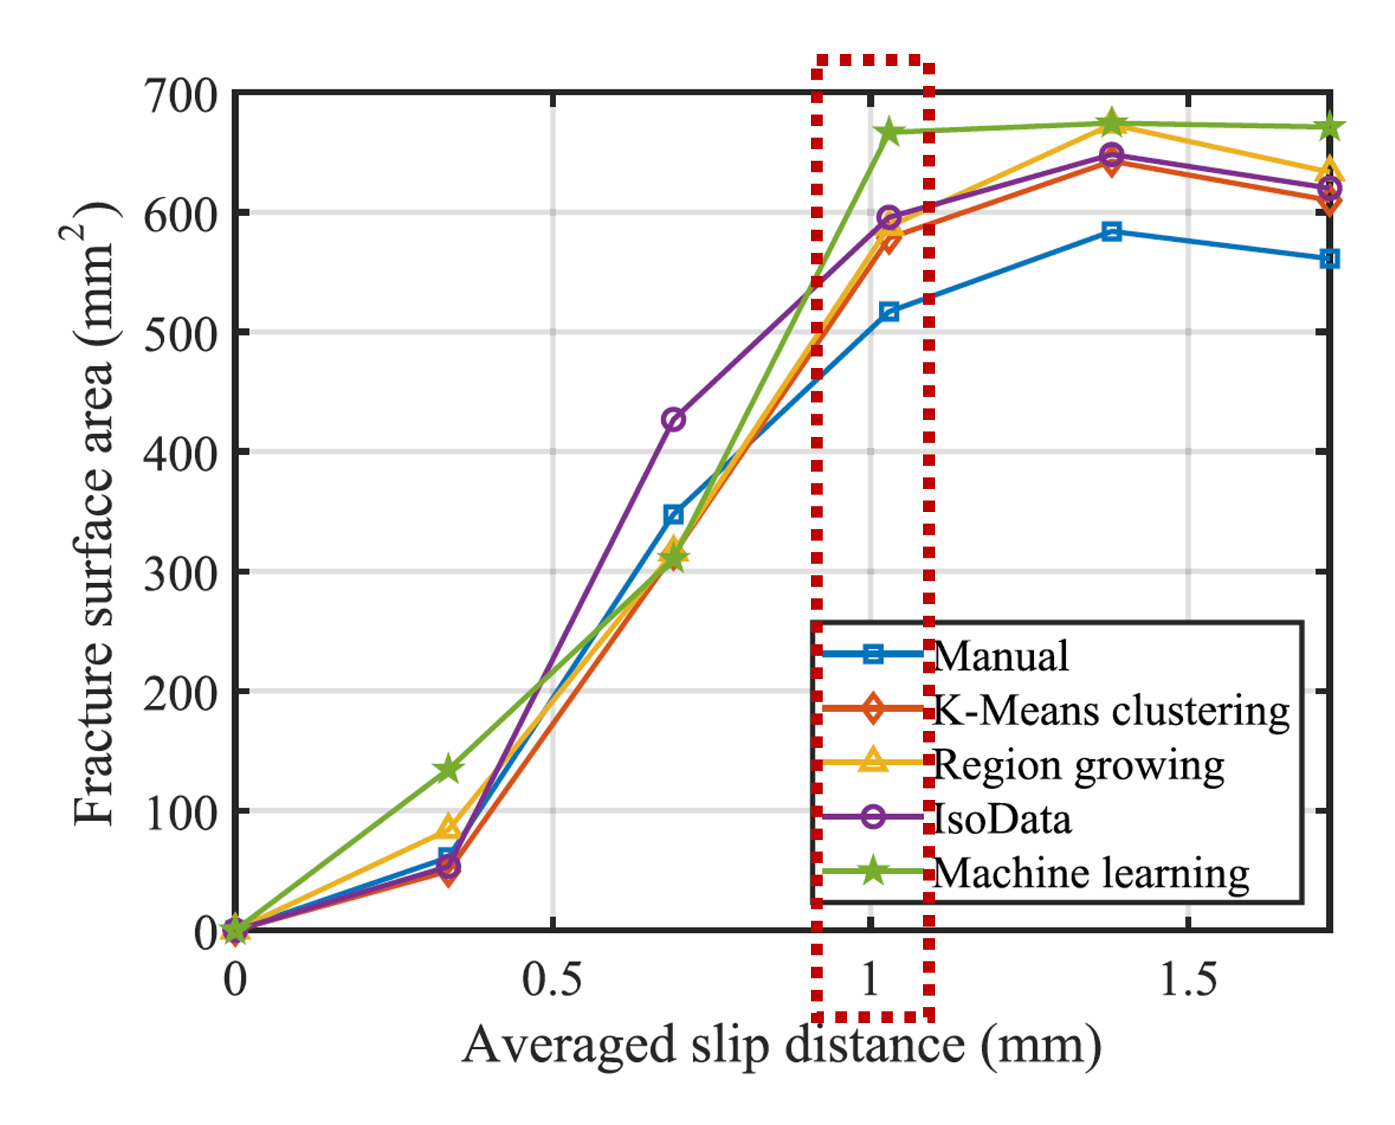
\includegraphics[width=0.4\textwidth]{Zhaoetal2020fig4.png}
\caption{Surface area calculations of the same images. After \cite[figure 4]{Zhao2020}}
\label{fig:Zhaoetal2020fig4}
\end{wrapfigure}

Since our data set and filtering kernels used in the convolution operation are made out of discrete values, the shape of the filter must be preserved. This means that when using the Matlab function \texttt{fspecial3} to generate the 3D filter, one needs to plot it and insure that the size of the filter results in second derivative filter shape that preserves the two-peak-one-trough shape for a specific scaling parameter $s$. To show this better, consider the 2D filter since it is easier to visualize. \Autoref{fig:Filters} shows the kernel generated using the \emph{gaussian} option of the Matlab function \texttt{fspecial2} (2D equivalent of \texttt{fspecial3}). Shown in this figure are four different filters for one scaling parameter $s = 1$. The filter sizes shown are 5, 9, 11, and 19. \Autoref{fig:Filter size 5} shows that the second derivative $G_{xx}$ shown in the right column does not preserver the trough-peak-trough shape required to produce the appropriate results. But a filter size of 9 or greater seem to preserve that shape, making such sizes sufficient to produce the correct results. The main advantage of keeping the filter size small however, is reducing the computing expense. For my synthetic images, which are 100 x 100 x 3 voxels in size, the computational time was minimal, but considering an actual image of a rock, the computations could become very expensive. An attempt that is not shown here on an image of size 1000 x 350 x 3 was made, and the computational time was about 15 minutes. This shows that there should be an optimal filter size for every scaling parameter $s$ to optimize the computational expense. 

\begin{figure}[!hb]
\centering
    \begin{subfigure}[b]{0.4\textwidth}            
            \includegraphics[width=\textwidth]{"s = 1, hSize = 5_normalized"}
            \caption{Filter size = 5}
            \label{fig:Filter size 5}
    \end{subfigure}%
     %add desired spacing between images, e. g. ~, \quad, \qquad etc.
      %(or a blank line to force the subfigure onto a new line)
    \begin{subfigure}[b]{0.4\textwidth}
            \centering
            \includegraphics[width=\textwidth]{"s = 1, hSize = 9_normalized"}
            \caption{Filter size = 9}
            \label{fig:Filter size 9}
    \end{subfigure}
    
    \begin{subfigure}[b]{0.4\textwidth}            
            \includegraphics[width=\textwidth]{"s = 1, hSize = 11_normalized"}
            \caption{Filter size = 11}
            \label{fig:Filter size 11}
    \end{subfigure}%
     %add desired spacing between images, e. g. ~, \quad, \qquad etc.
      %(or a blank line to force the subfigure onto a new line)
    \begin{subfigure}[b]{0.4\textwidth}
            \centering
            \includegraphics[width=\textwidth]{"s = 1, hSize = 19_normalized"}
            \caption{Filter size = 19}
            \label{fig:Filter size 19}
    \end{subfigure}
    
    \caption{Two-dimensional Gaussian filter $G(x,y)$ (top left of each set), and $G_{xx}(x,y)$ (top right of each set) for $s = 1$ and different filter sizes used in generating the kernels by the Matlab function \texttt{fspecial3}. The bottom row of each set is a traverse line along a line with y-axis value = 0.}
    \label{fig:Filters}
\end{figure}

\section{Conclusions and Future work}
The approach proposed by \cite{Voorn2013} seems to be successful at detecting fractures of multiple scales. There are a few parameters in the algorithm, such as the tolerance parameter $\gamma$ used in computing $C_s$ that require some trial and error to optimize the results. Further analysis on larger synthetic images and microCT rock images can be used to optimized the approach further. The size of the filters used in the computation of the Hessian are critical to produce correct results. The Hessian filtered images have the advantage of eliminating beam hardening, this is useful in consistently identifying isosurface values for surface area computations. Finally, further investigations into optimizing this approach to recover the fracture apertures is of value and will be considered in future work.

Furthermore, the Gaussian kernal used in \cite{Voorn2013} is isotropic. We anticipate that using an anisotropic Gaussian kernal has the potential of providing additional information about the fractures. The shape of an isosurface an anisotropic Gaussian kernal, i.e. 3D contour, yields a shape that has three principal directions of different magnitudes. This information can be utilized in identifying fracture orientation. This feature of fractures is helpful in understanding the extent of the fracture contribution in fluid flow within a rock sample. 


\clearpage
\newpage
\bibliographystyle{seg}
\bibliography{references}
\end{document}
